\label{sec::7_ah}
The second sub-objective within this thesis is now to close the control loop of figure \ref{fig::61_pg}, and to steer the robot towards desired goals, whilst avoiding obstacles. This requires a high-level command that arises from visual feedback. As discussed in the introductory section \ref{sec::1_in}, there are several ways to achieve this, among them human users, as shown in figure \ref{fig::7_cl}.
\begin{figure}[h!]
	\centering
	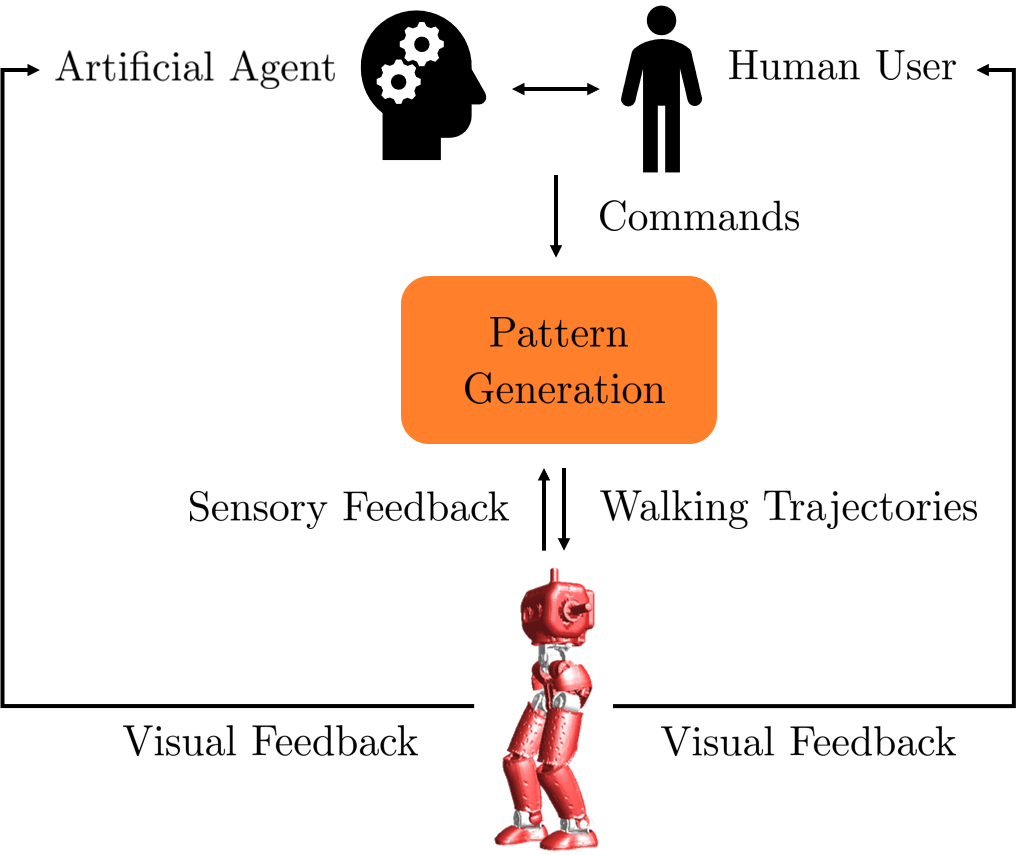
\includegraphics[scale=.5]{chapters/07_autonomous_high_level_control_of_the_walking_pattern_generator/img/control_loop.png}
	\caption{Proposed control loop to navigate the robot with either a human user or an artificial agent. The commands are given in the form of linear velocities $v_x$, and $v_y$, along the x-, and the y-axis, as well as an angular velocity $\omega_z$ about the z-axis of the robot's coordinates system. The building blocks of the pattern generation are shown in more detail in figure \ref{fig::61_pg}.}
	\label{fig::7_cl}
\end{figure}
Different approaches try to replace the human user via machine learning methods, which play a major role for autonomous navigation of robots, and whilst most recent approaches mainly dealt with tree search methods in 3D point-clouds, as highlighted in the introduction \ref{sec::1_in}, this thesis aims at utilizing neural networks for solving the task at hand. Neural networks are very promising for their low computational cost, and their ability to run with low energy usage on lightweight hardware, such as tensor processing units \cite{jouppi2017datacenter}, which is critical in the domain of humanoid robots. Neural networks may further enable one to combine spatial, semantic, and temporal understanding into one approach to achieve autonomous navigation, which is different to all existing methods. Within the following sections, two approaches of training neural networks for the desired task of autonomous navigation will, therefore, be presented. One of which clones the behavior of a human user (sec. \ref{sec::71_bc}), whereas the second presented reinforcement learning method (sec. \ref{sec::72_rl}) explores policies and tries to find solutions on its own. 